\pgfplotsset{width=11cm}
\renewcommand\arraystretch{1.5}
\subsection{TPH Testing in Air}
\begin{center}
\vspace{5mm}
\addcontentsline{lot}{table}{Table 1: TPH Calibration Data}
{\large {\bf Table 1: TPH Calibration Data\\}}
\vspace{2mm}
\begin{tabular}{|cc|}
    \hline
    \textbf{TPH Concentration~}$\left(\frac{\text{mg}}{\text{m}^3}\right)$ & \textbf{Air Quality (\%)}  \\\hline
    0.00001             & 0            \\
    0.0001              & 24           \\
    0.001               & 47           \\
    0.01                & 75           \\
    0.1                 & 96          \\\hline
\end{tabular}
\vspace{5mm}
\addcontentsline{lof}{figure}{Figure 1: TPH Calibration Curve}
\begin{tikzpicture}
    \begin{axis}[
        title={\textbf{Figure 1: TPH Calibration Curve}},
        xlabel={TPH Concentration (\(\frac{\text{mg}}{\text{m}^3}\))},
        ylabel={Air Quality (\%)},
        xmode=log,
        xmax=0.1, xmin=0.00001,
        ymin=0, ymax=100,
        ytick={0,25,50,75,100},
        ymajorgrids=true,
        grid style=dashed,
        legend pos = north west,
        legend cell align={left}
    ]
    
    \addplot[only marks, red] table [x=tph, y=air] {1.csv};
    \addplot[smooth, red, domain=0.00001:0.1] {10.553*ln(x)+121.3};
    \end{axis}
\end{tikzpicture}
\newpage

\addcontentsline{lot}{table}{Table 2: TPH Levels of Air Samples along Second Avenue}
{\large {\bf Table 2: TPH Levels of Air Samples along Second Avenue\\}}
\vspace{2mm}
\begin{tabular}{|cccc|}
    \hline
    \textbf{Street} & \textbf{TPH Deflection (\%)} & \textbf{Wind Speed (ft/min)} & \textbf{Temperature (\textsuperscript{o}F)}                           \\\hline
    13th            & 2                            & 720                          & 48.1                                                                  \\
    12th            & 0                            & 665                          & 47.1                                                                  \\
    11th            & 2                            & 877                          & 46.2                                                                  \\
    10th            & 2                            & 184                          & 47.4                                                                  \\
    9th             & 3                            & 305                          & 47.4                                                                  \\
    8th             & 3                            & 384                          & 47.2                                                                  \\
    7th             & 2                            & 189                          & 48.0                                                                  \\
    6th             & 2                            & 389                          & 48.2                                                                  \\\hline\hline
    \textbf{Street} & \textbf{Cars/Hour}           & \textbf{Air Quality TPH (\%)}    & \textbf{TPH Concentration~}$\left(\frac{\text{mg}}{\text{m}^3}\right)$  \\\hline
    13th            & 1380                         & 32                           & 0.00001050                                                            \\
    12th            & 1680                         & 30                           & 0.00001048                                                            \\
    11th            & 1340                         & 32                           & 0.00001050                                                            \\
    10th            & 1720                         & 32                           & 0.00001050                                                            \\
    9th             & 1340                         & 33                           & 0.00001051                                                            \\
    8th             & 1360                         & 33                           & 0.00001051                                                            \\
    7th             & 1320                         & 32                           & 0.00001050                                                            \\
    6th             & 1040                         & 32                           & 0.00001050 \\\hline                                                          
\end{tabular}
\vspace{5mm}
\addcontentsline{lof}{figure}{Figure 2: TPH Levels of Air Samples along Second Avenue}
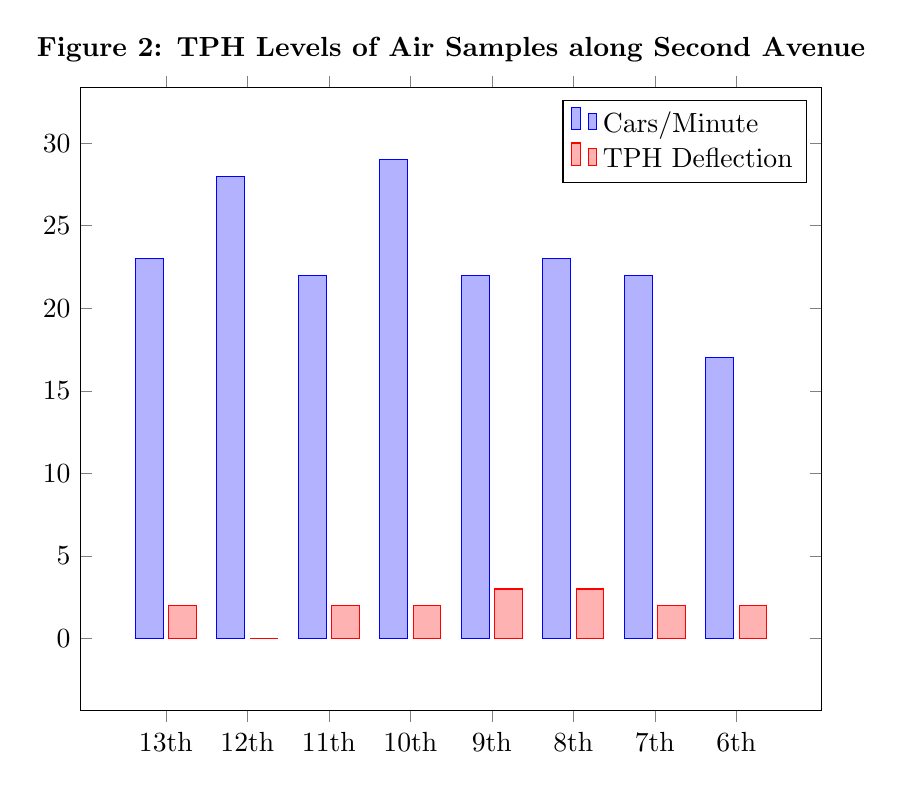
\begin{tikzpicture}
    \begin{axis}  
        [  
        title={\textbf{Figure 2: TPH Levels of Air Samples along Second Avenue}},
        ybar,  
        enlargelimits=0.15,  
        symbolic x coords={13th, 12th, 11th, 10th, 9th, 8th, 7th, 6th},
        xtick=data,  
        legend cell align={left}
        ]  
        \addplot coordinates {(13th,23) (12th,28) (11th,22) (10th,29) (9th,22) (8th,23) (7th, 22) (6th,17) };  
        \addplot coordinates {(13th,2) (12th,0) (11th,2) (10th,2) (9th,3) (8th,3) (7th, 2) (6th,2) };  
        \addlegendentry{Cars/Minute};  
        \addlegendentry{TPH Deflection};
        
    \end{axis}  
\end{tikzpicture}
\newpage

\addcontentsline{lot}{table}{Table 3: TPH Levels of Air Samples along Broadway}
{\large {\bf Table 3: TPH Levels of Air Samples along Broadway\\}}
\vspace{2mm}
\begin{tabular}{|cccc|}
    \hline
    \textbf{Street} & \textbf{TPH Deflection (\%)} & \textbf{Wind Speed (ft/min)} & \textbf{Temperature (\textsuperscript{o}F)}                           \\\hline
    13th   & 18                  & 125                 & 51.1                           \\
    12th   & 6                   & 210                 & 50.3                           \\
    11th   & 4                   & 53                  & 50                             \\
    10th   & 0                   & 118                 & 47.9                           \\
    9th    & 6                   & 43                  & 47.7                           \\
    8th    & -2                  & 228                 & 49.1                           \\\hline\hline
    \textbf{Street} & \textbf{Cars/Hour}           & \textbf{Air Quality TPH (\%)}    & \textbf{TPH Concentration~}$\left(\frac{\text{mg}}{\text{m}^3}\right)$  \\\hline
    13th   & 1540                & 66                  & 0.00001084                     \\
    12th   & 636                 & 54                  & 0.00001072                     \\
    11th   & 576                 & 52                  & 0.00001070                     \\
    10th   & 516                 & 48                  & 0.00001066                     \\
    9th    & 468                 & 54                  & 0.00001072                     \\
    8th    & 900                 & 46                  & 0.00001064 \\\hline                   
\end{tabular}
\vspace{5mm}
\addcontentsline{lof}{figure}{Figure 3: TPH Levels of Air Samples along Broadway}
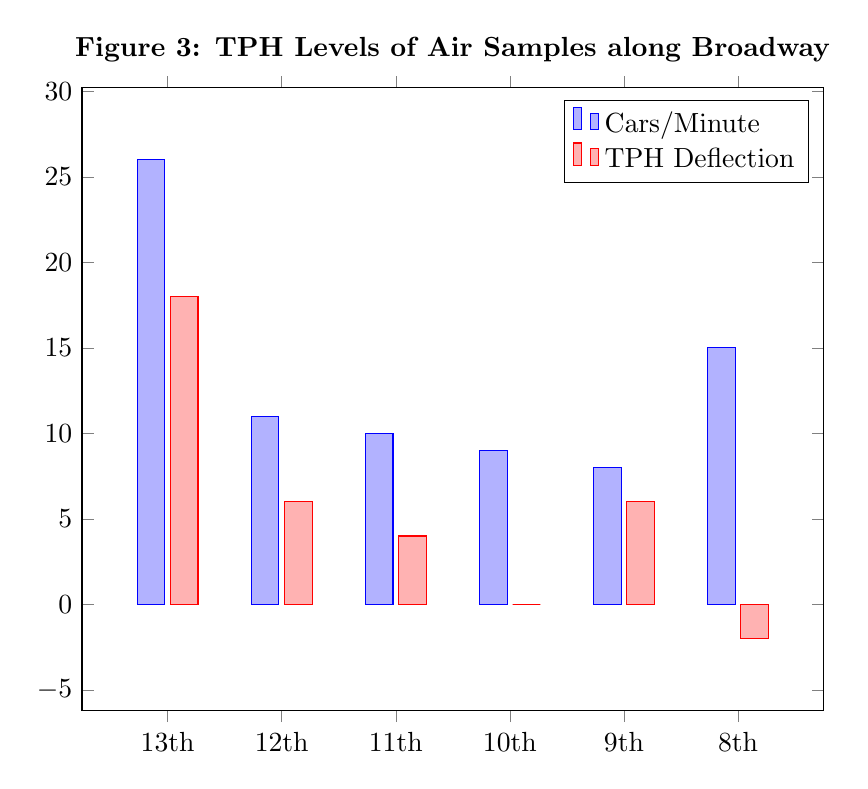
\begin{tikzpicture}
    \begin{axis}  
        [  
        title={\textbf{Figure 3: TPH Levels of Air Samples along Broadway}},
        ybar,  
        enlargelimits=0.15,  
        symbolic x coords={13th, 12th, 11th, 10th, 9th, 8th},
        xtick=data,  
        legend cell align={left}
        ]  
        \addplot coordinates {(13th,26) (12th,11) (11th,10) (10th,9) (9th,8) (8th,15)};  
        \addplot coordinates {(13th,18) (12th,6) (11th,4) (10th,0) (9th,6) (8th,-2) };  
        \addlegendentry{Cars/Minute};
        \addlegendentry{TPH Deflection};
        
          
    \end{axis}  
\end{tikzpicture}
\end{center}
\newpage
\subsection{PCB Testing in Soil}
\begin{center}
\vspace{5mm}
\addcontentsline{lot}{table}{Table 4: PCBs of Soils Collected Locally}
{\large {\bf Table 4: PCBs of Soils Collected Locally\\}}
\vspace{2mm}
\begin{tabular}{|cccccc|}
    \hline
    \textbf{Location}     & \textbf{Initials} & \textbf{Color} & \textbf{Solvent (mL)} & \textbf{Mass (g)} & \textbf{PCB (ppm)}  \\\hline
    Peter Cooper Triangle & EE                & Peach          & 2.5                             & 10                     & 108                 \\
    Peter Cooper Triangle & JM                & Yellow         & 6                               & 10                     & 50                  \\
    Peter Cooper Triangle & SS                & Purple         & 6                               & 10                     & 25                  \\
    Peter Cooper Triangle & GR                & Purple         & 6                               & 10                     & 30                  \\
    Peter Cooper Triangle & RE                & Purple         & 6                               & 10                     & 25                  \\
    Peter Cooper Triangle & HC                & Purple-Yellow  & 6                               & 10                     & 45                  \\
    7th and Cooper Sq     & SZ                & Light Purple   & 5                               & 10                     & 36                  \\
    Peter Cooper Statue   & DT                & Purple         & 5                               & 10                     & 30                  \\
    Peter Cooper Statue   & AD                & Light Purple   & 6                               & 10                     & 30                  \\
    7th and 2nd           & JS                & Light Pink     & 6                               & 10                     & 35                  \\
    6th and 2nd           & SC                & Light Purple   & 5                               & 10                     & 36                  \\
    Peter Cooper Statue   & HC                & Purple-Pink    & 5                               & 10                     & 42                  \\
    8th Floor Terrace     & AT                & Purple         & 2                               & 10                     & 75                  \\
    8th Floor Terrace     & PM                & Purple         & 2.5                             & 10                     & 72                  \\
    8th Floor Terrace     & SH                & Light Purple   & 5                               & 10                     & 48                  \\
    Peter Cooper Triangle & JK                & Purple         & 5                               & 10                     & 42                  \\
    5th and Bowery        & DM                & Magenta        & 5                               & 10                     & 48\\\hline           
\end{tabular}
\end{center}
\newpage
\subsection{TPH Testing in Soil}
\begin{center}
\vspace{5mm}
\addcontentsline{lot}{table}{Table 5: TPH Levels of Soils Throughout New York City}
{\large {\bf Table 5: TPH Levels of Soils Throughout New York City\\}}
\vspace{2mm}
\begin{tabular}{|ccccc|}
    \hline
    \textbf{Location}           & \textbf{Initials} & \textbf{Mass (g)} & \textbf{TPH (ppm)} & \textbf{Actual TPH (ppm)}  \\\hline
    Schiff Park                 & GR                & 10                & 349                        & 349                                \\
    East River South            & JS                & 9.9               & 1263                       & 1250.37                            \\
    Gobonda Playground          & RJ                & 10                & 628                        & 628                                \\
    Jacob's Ladder Playground   & SC                & 10                & 412                        & 412                                \\
    Ancient Playground          & SH                & 10                & 96                         & 96                                 \\
    Sachkerah Woods Playground  & GR                & 10.1              & 355                        & 358.55                             \\
    Rudin Playground            & JM                & 10                & 1587                       & 1587                               \\
    Magenta Playground          & JS                & 10.1              & 773                        & 780.73                             \\
    Battery Park                & JM                & 10.1              & 620                        & 626.2                              \\
    110th and Lenox             & RJ                & 10                & N/A                        & N/A                                \\
    Rudin Playground            & SC                & 10                & 1373                       & 1373                               \\
    Fort Independent Playground & SH                & 10                & 821                        & 821                                \\
    Sachkerah Woods Playground  & HC                & 10                & 336                        & 336                                \\
    Sycamore's Park             & SZ                & 10                & 1506                       & 1506                               \\
    Cooper Square Park          & EE                & 10                & 1373                       & 1373                               \\
    Cooper Square Park          & DM                & 10                & 448                        & 448                                \\
    Cooper Square Park          & NS                & 10                & 229                        & 229                                \\
    Cooper Square Park          & PM                & 10                & 431                        & 431 \\\hline                              
    \end{tabular}
\end{center}
